\subsection{Inneres Kongobecken: \textit{Äquator-Co-Tradition}}\label{sec:ICB_StilGrDatierungen}

Die von \textcite{Wotzka.1995} für das Innere Kongobecken erarbeitete Sequenz aus keramischen Stilen liefert erstmals eine umfassende Übersicht über die Entwicklungslinien und darauf aufbauende Rückschlüsse auf den Besiedlungsgang dieser östlich an das Arbeitsgebiet angrenzenden Großregion. Die Sequenz Wotzkas basiert auf einem relativchronologischen System aus typologischen Verkettungen, das mit absolutchronologischen Kalibrationspunkten erweitert wurde. Im Folgenden sollen die jeweiligen Synthesen Wotzkas zur zeitlichen Einordnung der 34 von ihm beschriebenen Stilgruppen aus dem Inneren Kongobecken knapp referiert werden. \textcite[]{Wotzka.1995} kondensiert die sich aus den einzelnen Stilgruppen ergebenden typologischen Abhängigkeiten zu sechs Stiltradtionen, von denen fünf genealogisch zusammenhängen und die \textit{Äquator-Co-Tradition} bilden \textsc{Wotzka} (ebd. 222 Abb.~4).

Für den ältesten, im Inneren Kongobecken nachgewiesenen Keramikstil, die Imbonga-Gruppe, kommt \textsc{Wotzka} (ebd. 67) zu dem Schluss, dass die \enquote{akzeptablen Datierungen in den Zeitraum zwischen etwa 400 und 100 v.~Chr. fallen}. Von insgesamt zwölf aus Imbonga-Kontexten stammenden Radiokohlenstoffdatierungen (ebd. 67 Tab.~9; Tab.~\ref{tab:Wotzka1995-412_14C_Repr}) können lediglich sechs als repräsentativ angesehen werden, während zwei Datierungen (Hv-11574, Hv-12627) deutlich zu alt und vier Daten (Hv-11571, Hv-11573, GrN-13586, KN-4205) zu jung ausfallen, um akzeptiert werden zu können.\footnote{Die urprüngliche Definition der Imbonga-Gruppe durch \textcite{Eggert.1983} umfasste auch das von \textcite{Wotzka.1995} den Stilgruppen Bonkake, Ingende und Inganda zugewiesene Formenspektrum. Siehe auch Anm.~\ref{ftn:AufteilungIMB}.} Die Keramik der Bonkake-Gruppe könne als \enquote{teilweise mit einer fortgeschrittenen Phase des Imbonga-Stiles identisch} angesehen werden (ebd. 72). Für sie kann folglich ein Zeitraum von der Mitte des 3.~Jh. bis in das 1.~Jh. v.~Chr. als Datierung vorgeschlagen werden. Die ebenfalls \enquote{in etwa zeitgleiche, teilweise mit dem Imbonga-Stil parallele} Ingende-Gruppe überdauert nach \textsc{Wotzka} (ebd. 88) das Ende von Imbonga um etwa 100 v.~Chr.

\begin{figure*}[p]
	\centering
	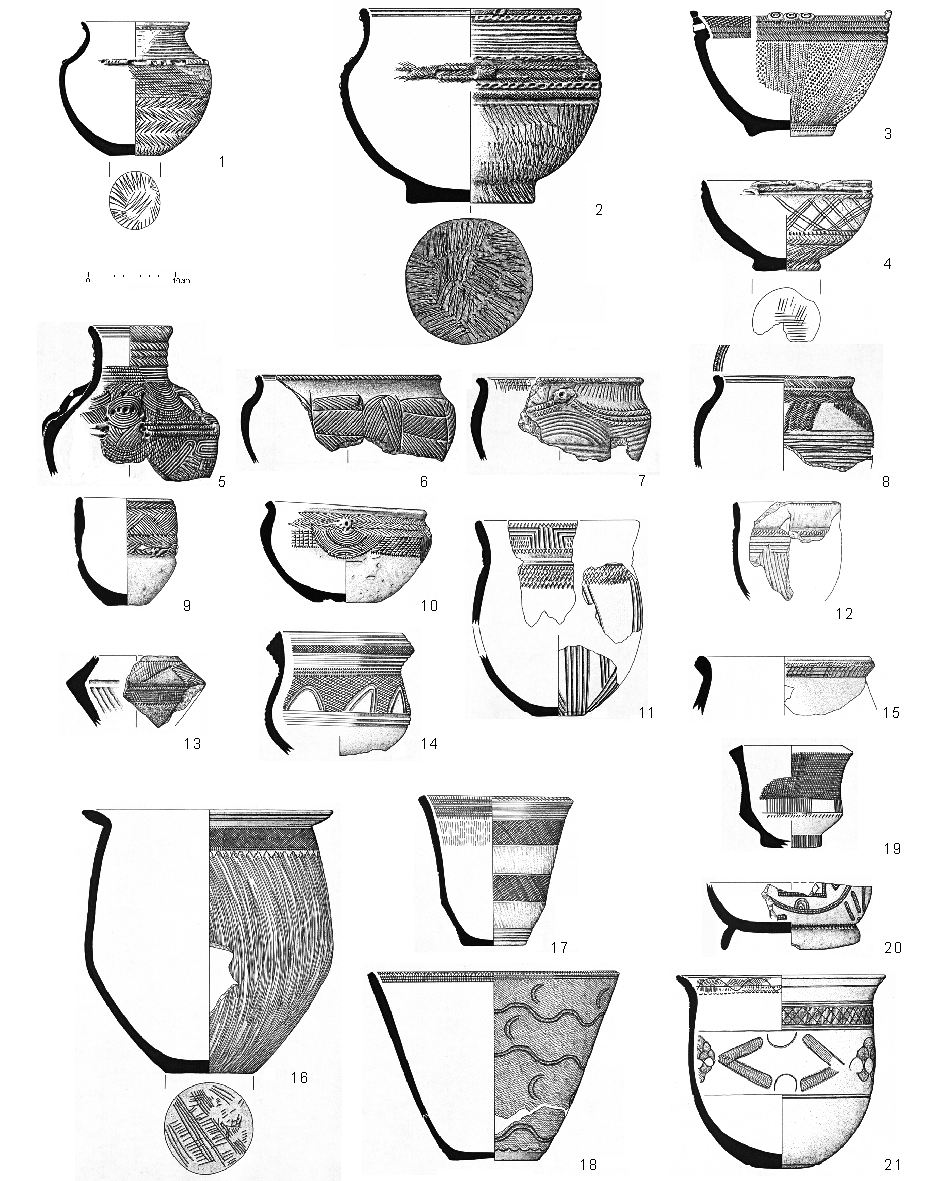
\includegraphics[width = \textwidth]{fig/InneresKongobecken_Typen_ICB_EIA1-3.pdf}
	\caption{Inneres Kongobecken: Typvertreter des ältere Abschnitts (4.~Jh. v.~Chr.--7.~Jh. n.~Chr.)  der \textit{Äquator-Co-Tradition} nach \textcite{Wotzka.1995}.\\1--4: Imbonga-Gruppe (ebd. 453 Taf.~19.5, 490 Taf.~56.2, 496 Taf.~62.10, 453 Taf.~19.6); 5--6: Bonkake-Gruppe (ebd. 495 Taf.~61.6, 495 Taf.~61.8); 7--8: Ingende-Gruppe (ebd. 479 Taf.~45.1, 484 Taf.~50.1); 9--10: Inganda-Gruppe (ebd. 472 Taf.~38.3, 472 Taf.~38.4); 11--12: Lokondolo-Gruppe (ebd. 500 Taf.~66.16, 455 Taf.~21.6); 13--14: Yete-Gruppe (ebd. 505 Taf.~71.9, 505 Taf.~71.14); 15: Monkoto-Gruppe (ebd. 487 Taf.~53.4); 16: Bokele-Gruppe (ebd. 454 Taf.~20.7); 17--18: Lingonda-Gruppe (ebd. 510 Taf.~76.10, 511 Taf.~77.4); 19: Lusako-Gruppe (ebd. 485 Taf.~51.3); 20--21: Bokuma-Gruppe (ebd. 526 Taf.~92.5, 474 Taf.~40.4a).}
	\label{fig:Wotzka1995_TypenICB_EIA1}
\end{figure*}

\begin{figure*}[tb!]
	\centering
	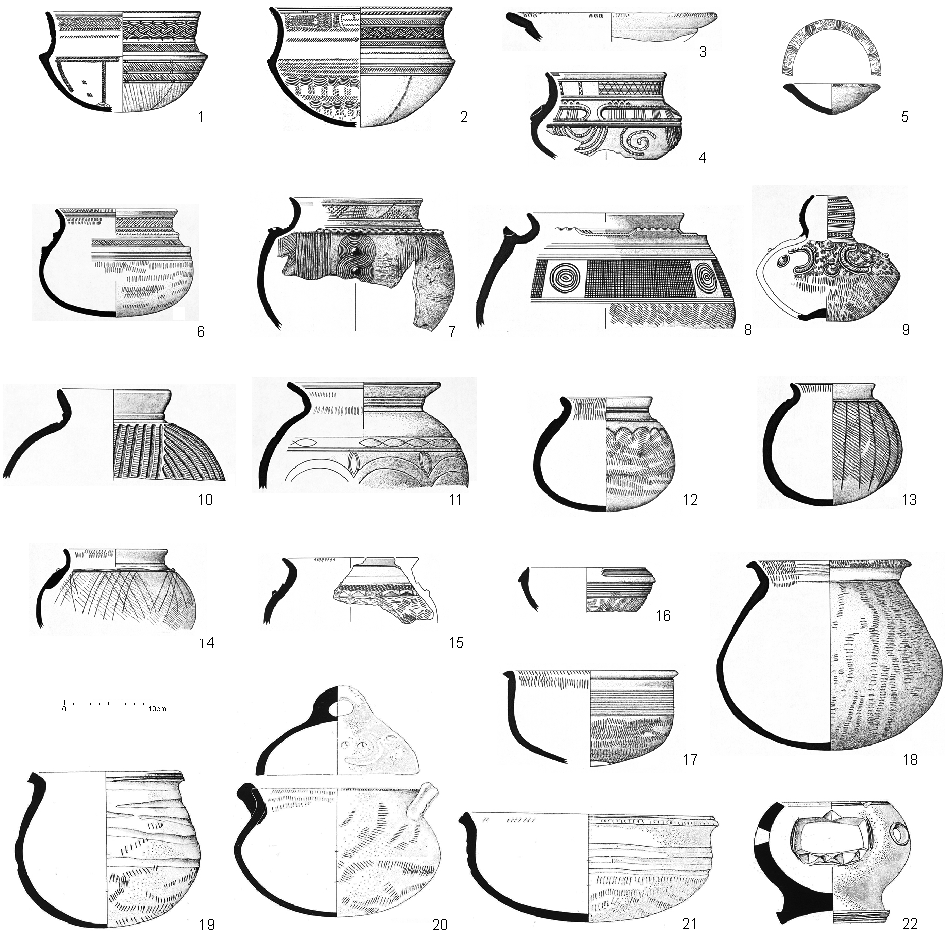
\includegraphics[width = \textwidth]{fig/InneresKongobecken_Typen_ICB_LIA1-3.pdf}
	\caption{Inneres Kongobecken: Typvertreter des jüngeren Abschnitts (11.--20.~Jh. n.~Chr.) der \textit{Äquator-Co-Tradition} nach \textcite{Wotzka.1995}.\\1--3: Longa-Gruppe (ebd. 485 Taf.~51.9, 485 Taf.~51.10, 531 Taf.~97.8); 4--9: Bondongo-Gruppe (ebd. 532 Taf.~98.4, 445 Taf.~11.3, 443 Taf.~9.17, 521 Taf.~87.7, 490 Taf.~56.1, 449 Taf.~15.1); 10--11: Mbandaka-Gruppe (ebd. 446 Taf.~12.2, 446 Taf.~12.1); 12--13: Nkile-Gruppe (ebd. 527 Taf.~93.4, 531 Taf.~97.7); 14--15: Besongo-Gruppe (ebd. 509 Taf.~75.4, 522 Taf.~88.4); 16--18: Botendo-Gruppe (ebd. 458 Taf.~24.5, 482 Taf.~48.6, 481 Taf.~47.2); 19--22: Ikenge-Gruppe \parencite[427 Abb.~23.5, 426 Abb.~22.1a--b, 428 Abb.~24.2, 429 Abb.~25.2]{Eggert.1980c}.}
	\label{fig:Wotzka1995_TypenICB_LIA1}
\end{figure*}

Die Keramik der Inganda-Gruppe setzt \textsc{Wotzka} (ebd. 84) \enquote{aufgrund stilistischer Erwägungen im Wesentlichen [als] jünger} als das Material der Bonkake- und Ingende-Gruppe an. Es zeige sich jedoch eine \enquote{stilistische Nähe zwischen Imbonga- und Bonkake-Gruppe einerseits und Bonkake- und Inganda-Gruppe andererseits} (ebd.), welche als Effekt einer zeitlichen Nähe der besagten Gruppen anzusehen sei. Drei übereinstimmende Radiokarbondaten für die Inganda-Gruppe aus Bokuma (ebd. 84 Tab.~22; Tab.~\ref{tab:Wotzka1995-412_14C_Repr}) \enquote{umfassen einen Gesamtzeitraum zwischen 196 v.~Chr. und 80 n.~Chr.} und belegten für Wotzka die relativ-chronologischen Beobachtungen für die Datierung der Inganda-Keramik. Stilistisch eng mit der Inganda-Keramik verbunden, zeige das Fundmaterial der Lokondola-Gruppe Ähnlichkeiten zu jüngeren Stilgruppen und müsse \enquote{als [ein] im Wesentlichen später als die Inganda-Gruppe zu datierendes Phänomen gelten} (ebd. 89). Die Keramik der Yete-Gruppe weise einerseits zwar deutliche Ähnlichkeiten zum Material der Lokondola-Gruppe auf, andererseits seien die Verbindungen zur Inganda-Gruppe jedoch unspezifischer (ebd. 93). Wie die Lokondola-Keramik, zeige auch das Yete-Material Ähnlichkeiten zu jüngeren Gruppen wie die Bokuma- und Lingonda-Gruppe, so dass \enquote{Lokondola- und Yete-Stil zunächst als mehr oder minder zeitgleiche Phänomene} aufgefasst werden können (ebd. 94).

Wotzka (ebd. 99) zufolge lässt sich für den Monkoto-Stil \enquote{eine sowohl der Lokondola- als auch der Yete-Gruppe benachbarte, im Wesentlichen aber nach diesen beiden Stilgruppen anzusetzende chronologische Position} postulieren. In der relativ-chronologischen Betrachtung sieht \textsc{Wotzka} (ebd.) zeitliche Überschneidungen dieser drei Stilgruppen als sehr wahrscheinlich an. Aus Kontexten mit Fundgut der Monkoto-Gruppe liegen fünf Radiokohlenstoffdatierungen vor (ebd. 99 Tab.~32; Tab.~\ref{tab:Wotzka1995-412_14C_Repr}), von denen nach Wotzkas Betrachtung allein das jüngste Datum (Hv-12613), welches kalibriert einen Zeitraum vom 1.~Jh. v.~Chr. bis zum 2.~Jh. n.~Chr. abdeckt, als repräsentativ angesehen werden kann. Die Keramik der Bokele-Gruppe sei etwa zeitgleich zu jener des Monkoto-Stils (ebd. 103). Aufgrund von Fundvergesellschaftungen am Fundplatz Bokele (Fpl.~14) sei \enquote{eine Überschneidung der Laufzeiten von Bokele-, \mbox{Lingonda-,} Longa-, und Mbandaka-Keramik [...] belegt} sowie durch stilistische Ähnlichkeiten zwischen den Gruppen Bokele-, Lokondola- und Yete-Gruppe als wahrscheinlich anzusehen (ebd. 103). Ein Radiokohlenstoffdatum aus einer Deponierung mit Bokele- sowie Lingonda-Keramik in Bokele liefert die einzige absolut-chronologische Referenz für die Keramik der Bokele-Gruppe (ebd. 312 Kat.-Nr.~9; Tab.~\ref{tab:Wotzka1995-412_14C_Repr}). Das Datum (KN-4204) deckt einen Zeitraum vom \mbox{1.--3.~Jh.} n.~Chr. ab, was nach \textsc{Wotzka} (ebd. 104) \enquote{vorläufig grob die ersten beiden nachchristlichen Jahrhunderte als Epoche des Bokele-Stiles} wahrscheinlich macht.

Die Keramik der Lusako-Gruppe wird von Wotzka (ebd. 106\,f.) \enquote{im Wesentlichen [als] später als der Inganda-Stil und in etwa zeitgleich mit dem Lokondola- und dem Yete-Stil} angesehen. Das einzige für die Lusako-Keramik repräsentative Radiokohlenstoffalter stammt aus dem Grabungsbefund PIK~87/1 in Pikunda am \mbox{Sangha}, der erst im Rahmen dieser Arbeit vollständig aufgearbeitet wurde (Kat.-Nr.~8). Das betreffende Datum (KI-2877) deckt einen Zeitraum vom späten 2.~Jh. v.~Chr. bis in die Mitte des 3.~Jh. n.~Chr. ab. Dieser deckt sich mit denen von \textsc{Wotzka} (ebd. 107) für die Keramik der Inganda-Gruppe präsentierten drei Datierungen und stützt somit den relativ-chronologischen Ansatz der Lusako-Gruppe. Für die Keramik der Lingonda-Gruppe liegen sechs Radiokohlenstoffdatierungen vor, von denen lediglich drei (GrN-14004, GrN-13076, KN-4206) den von \textsc{Wotzka} (ebd. 115 Tab.~44; Tab.~\ref{tab:Wotzka1995-412_14C_Repr}) erarbeiten chronologischen Ansatz stützen. Generell nimmt \textsc{Wotzka} (ebd. 115) für die Lingonda-Keramik eine Datierung \enquote{zwischen der jüngeren Hälfte des dritten und der Mitte des siebten Jahrhunderts} an. Als zeitgleich zur Lingonda-Keramik sieht er (ebd. 120) die Funde der Bokuma-Gruppe. Die Fundvergesellschaftung mit Material der Stilgruppen Inganda, Lokondola und Lingonda innerhalb des Grabungsbefunds BOK~85/3 (ebd. 330--331 Kat.-Nr.~20) zeige eine \enquote{partielle Überschneidung der Laufzeiten der in dem genannten Befund assoziierten Stilgruppen} (ebd. 120). Absolut-chronologische Ansätze liefern lediglich eine Datierung, die einen Zeitraum vom \mbox{3.--5.~Jh.} n.~Chr. abdeckt (ebd. 120; Tab.~\ref{tab:Wotzka1995-412_14C_Repr}).

Die Longa-Gruppe bildet das stilistische Bindeglied zwischen den bereits besprochenen Stilgruppen der Älteren Eisenzeit und den im Folgenden zu erörternden jüngeren Stilen. \textsc{Wotzka} (ebd. 127) konstatiert, dass die Keramik der Longa-Gruppe \enquote{stilistisch problemlos an das jüngere Ende der bisher entwickelten Keramiksequenz anzubinden ist}. Die Longa-Gruppe weise aber auch Parallelen zu den Stilen Bokuma und Bokele auf, die generell dem älteren Abschnitt der Keramiksequenz zuzurechnen sind. Auf der anderen Seite würden die noch deutlicheren Ähnlichkeiten zur Bondongo-Keramik auf ein jüngeres Alter des Longa-Materials hindeuten (ebd.). Aus Kontexten mit Fundgut der Longa-Gruppe stammen drei sehr unterschiedliche Radiokohlenstoffdatierungen (ebd. 127 Tab.~53, 128; Tab.~\ref{tab:Wotzka1995-412_14C_Repr}), die keine verbindliche absolut-chronologische Einordnung erlauben.\footnote{Im Jahr 2015 von H.-P. Wotzka veröffentlichte Typentafeln für die Stilgruppen des Innen Kongobeckens (siehe \url{http://www.fstafrika.phil-fak.uni-koeln.de/22669.html}; Stand 01.\,02.\,2016) weisen -- wo bekannt -- auch die chronologische Position aus. Für die Longa-Gruppe gibt Wotzka einen möglichen Zeitraum vom 12./13.~Jh. n.~Chr. an. Dieser wird durch keine neueren Datierungen getragen, er spiegelt vielmehr eine andere Gewichtung der starken typologischen Bezüge der Longa-Keramik zur Bondongo-Keramik wider. Damit verbunden scheint Wotzka nunmehr der Ansicht zu sein, dass die jüngste der drei vorliegenden Radiokohlenstoffdatierungen (\textsc{Wotzka} 1995: 127 Tab.~53: Hv-11572) als eher repräsentativ für die Longa-Gruppe anzusehen ist.\label{ftn:fstafrikaWebStilGr-Tafeln}} Innerhalb der von \textsc{Wotzka} (ebd. 222 Abb.~4) erarbeiteten Sequenz keramischer Stile nimmt die Longa-Gruppe eine Sonderstellung ein, da sie als einzige die Merkmale der älteren Stile mit jenen der jüngeren Phase verbindet. Jedoch werfen die stärkeren Ähnlichkeiten zu jüngeren Stilen und die problembehafteten absoluten Datierungen gegenwärtig Zweifel an der von \textsc{Wotzka} (ebd. 65, 221, 274, 285) postulierten ungebrochenen Traditionslinie auf.

Neben der Imbonga-Keramik stellt die Keramik der Bondongo-Gruppe die am besten durch absolute Daten chronologisch abgesicherte Stilgruppe des Inneren Kongobeckens dar. Neun der insgesamt 14 vorliegenden Datierungen (ebd. 138 Tab.~58; Tab.~\ref{tab:Wotzka1995-412_14C_Repr}), die einen Zeitraum zwischen dem Beginn des 11. Jh. bis zum Ende des 14 Jh. n.~Chr. abdecken, werden von Wotzka als repräsentativ für die Stilgruppe angesehen (ebd. 138). Im Fall der Mbandaka-Gruppe sprächen \enquote{sowohl die Grabungsergebnisse von Mbandaka als auch die engen Stilbezüge zwischen Mbandaka- und Bondongo-Keramik für eine weitgehende oder sogar vollständige zeitliche Kongruenz beider Stilgruppen} (ebd. 143). Während keine Radiokohlenstoffdatierung ausschließlich mit Keramik des Mbandaka-Stils assoziiert ist, wurde im Zusammenhang mit vier Datierungen -- neben anderen Stilen -- auch Mbandaka-Keramik gefunden (Tab.~\ref{tab:Wotzka1995-412_14C_Repr}). Während eine Datierung ein deutlich zu junges Datum lieferte (Hv-11578), decken die drei übrigen Datierungen (KI-2364, Hv-11572, Hv-12206) das 11.--14.~Jh. n.~Chr. ab und stützen die zeitliche Überschneidung mit der Bondongo-Gruppe. Von stilistischer Seite aus bleiben für Wotzka Zweifel an einer \enquote{unmittelbaren chronologischen Nachbarschaft} (ebd. 149) der Keramik der Nkile-Gruppe zu jener der Bondongo-Gruppe. Auch \enquote{stellt die Nkile-Gruppe ein stilistisches Bindeglied zwischen der Bondongo- und der Botendo-Keramik dar} (ebd. 149). Absolut-chronologisch könne die Nkile-Gruppe lediglich auf der Basis eines Datums (Hv-8916) aus der namensgebenden Fundstelle Nkile (Fpl.~17) eingeordnet werden, welches einen Zeitraum vom Ende des 13. bis zum Ende des 14. Jh. n.~Chr. abdeckt (ebd. 150; Tab.~\ref{tab:Wotzka1995-412_14C_Repr}). Neben Fundmaterial der Nkile-Gruppe repräsentiert dieses Datum jedoch auch Keramik der Bondongo-Gruppe. Die bereits erwähnte Botendo-Keramik stelle relativ- wie auch absolut-chronologisch ein jüngeres Phänomen dar, es handele sich um die zeitgenössische Keramik des sogenannten \textit{Musée du Congo} (ebd. 157). Vertreter dieses Stils konnten von \textsc{Wotzka} (ebd. 157) in der Veröffentlichung ethnografischen Fundmaterials aus dem ehemaligen \textit{Unabhängigen Freistaat Kongo} \parencite[155--157 Taf.~12]{Coart.1907} identifiziert werden. Zwei Radiokohlenstoffdatierungen aus der Grabung NKI~2 in Nkile \parencite[Fpl.~17; ][158 Tab.~70, 318--322 Kat.-Nr.~13; Tab.~\ref{tab:Wotzka1995-412_14C_Repr}]{Wotzka.1995} ergaben ein rezentes Probenalter (Hv-9562). Die zweite Probe (Hv-9561) deckt einen Zeitraum zwischen dem Ende des 17.~Jh. bis in rezente Zeiten ab. Den Abschluss der für den westlichen Teil des Inneren Kongobeckens von Wotzka erarbeiteten Sequenz, den er unter der Bezeichnung \textit{West-Tradition} subsumiert (ebd. 221\,f.), bildet die Keramik aus Ikenge (Fpl.~20), deren Herstellung im Zuge des \textit{River Reconnaissance Project} 1977 \parencite{Eggert.1980c} und in den 1980er Jahren beobachtet werden konnte.

Die chronologische Einordnung der keramischen Stilgruppen der Traditionen \textit{Luilaka}, \textit{Tshu"-a"-pa}, \textit{Busira}, \textit{Maringa} sowie der sogenannten \textit{Nord-Tradition} \parencite[221--224]{Wotzka.1995} fiel aufgrund mangelnder Radiokohlenstoffdatierungen in vielen Fällen schwerer. Für die der \textit{Luilaka-Tradition} zugerechnete Bekongo-Gruppe sieht \textsc{Wotzka} (ebd. 162) anhand stilistischer Erwägungen \enquote{eine Zeitstellung im chronologischen Überschneidungsbereich zwischen Longa- und Bondongo-Stil} jedoch keine \enquote{vollständige zeitliche Kongruenz mit dem Longa-Stil} und auch keine \enquote{komplette Parallelisierung mit der Bondongo-Gruppe}. Für die Wafanya-Gruppe stehe von stilistischer Seite \enquote{eine besondere Nähe zur Bondongo-Gruppe außer Frage} (ebd. 167), so dass eine zeitliche Parallelität mit dem \textit{klassischen} Bondongo sehr wahrscheinlich scheine. Darüber hinaus kann laut Wotzka als sicher gelten, dass sie zeitlich direkt auf die Bekongo-Gruppe folgt. \textsc{Wotzka} (ebd.) sieht in der Keramik der Wafanya-Gruppe \enquote{keine generell späte, sondern vielmehr eine über längere Zeit parallel bestehende, lokale Fazies des Bondongo-Stiles}. 

Den Beginn der \textit{Tshuapa-Tradition} bildet die Keramik der Wema-Gruppe. Bei ihr handele es sich stilistisch gesehen um eine \enquote{späte, formal und ornamental stark vereinfachte Ausprägung der Bondongo-Keramik} (ebd. 171). Lediglich eine der drei vorliegenden Radiokohlenstoffdatierungen aus Kontexten mit Wema-Keramik (ebd. 171 Tab.~81; Tab.~\ref{tab:Wotzka1995-412_14C_Repr}) können nach Wotzkas Ansicht als repräsentativ für die Stilgruppe angesehen werden. Dieses eine Datum (GrN-13078) deckt einen Zeitraum vom \mbox{13.--14.~Jh.} n.~Chr. ab (ebd. 172). Zwischen die Keramik der Wema-Gruppe und jener der jüngeren Bolondo-Gruppe sei das Material der Bosanga-Gruppe zu verorten, welches zudem eine \enquote{stilistisch und stratigrafisch zu begründende Gleichzeitigkeit mit der Nkile-Gruppe} aufweise (ebd. 175). Wie im Fall der Wema-Gruppe, stehen auch für die Keramik der jüngeren Bolondo-Gruppe drei Radiokohlenstoffdatierungen zur Verfügung (ebd. 180 Tab.~88; Tab.~\ref{tab:Wotzka1995-412_14C_Repr}), von denen Wotzka (ebd. 181) jedoch lediglich das jüngste, bis mindestens in das 16.~Jh. zurückreichende Datum (KN-4203) als repräsentativ ansieht. Die beiden älteren Datierungen (Hv-12618, Hv-12625) ließen sich nicht mit der erarbeiten relativ-chronologischen Gliederung vereinen. Für die Bokone-Gruppe stellt Wotzka (ebd. 185) zusammenfassend fest, dass sie eine \enquote{sowohl stratigrafisch als auch stilistisch zu begründende relativ-chronologische Stellung zwischen dem Bolondo-Stil und der rezenten Ilemba-Bokonda-Keramik des Tshuapa-Gebietes} einnimmt. Dem Fundgut der Bokone-Gruppe ließen sich keine Radiokohlenstoffdatierungen zuordnen. Ebenfalls ohne absolut-chronologische Daten konnte für die Keramik der Bolombi-Gruppe \enquote{unter der Prämisse, dass es sich nicht um eine speziell verzierte Fazies der rezenten Tshuapa-Keramik handelt}, nur eine \enquote{relativ-chronologische Position zwischen dem Bokone- und dem Ilemba-Bokonda-Stil} postuliert werden (ebd. 187). Die Keramik der Ilemba-Bokonda-Gruppe repräsentiert die \enquote{rezente Töpferei des unteren Tshuapa-Gebietes} (ebd. 188) wie sie bei den Feldaufenthalten des \textit{River Reconnaissance Project} im Jahr 1983 noch beobachtet werden konnte.

Die der \textit{Busira-Tradition} zugerechnete Keramik der Inkaka-Gruppe ließ sich nicht zweifelsfrei relativ-chronologisch einordnen. Basierend auf stilistischen Ähnlichkeiten sowie den Fundumständen eines Gefäßes aus Ngombe-Malala (Fpl.~89) schließt \textsc{Wotzka} (ebd. 196) auf eine \enquote{grundsätzlich subrezente Zeitstellung der Inkaka-Gruppe}. Die der Liyolongo-Gruppe zugerechnete Keramik spiegelt die 1983 beobachtete \enquote{rezente Töpferei in Liyolongo [Fpl.~85] am mittleren Busira} (ebd.) wider und bildet den rezenten Abschluss der keramischen Sequenz in dieser Region des Inneren Kongobeckens. Die rezente Töpferei im Bereich des oberen Maringa wurde 1985 in Yopoko beobachten und dokumentiert (Fpl.~175; ebd. 197). 

Neben den referierten Stilgruppen definierte \textcite{Wotzka.1995} in dem von ihm untersuchten Fundgut einige stilistische und formale Einheiten, denen er zwar eigene Stilgruppen-Be"-zeich"-nungen gab, die aber eher regionale Ausprägungen überregionaler Gruppen darstellen. Eine dieser Gruppen ist die Lokongo-Gruppe, die \enquote{als regional geprägte Fazies des wesentlich weiträumiger verbreiteten Botendo-Stiles} (ebd. 200) angesehen werden kann. Die Malelembe-Gruppe hingegen kann als \enquote{lokale Variante des Nkile-Stiles} (ebd. 201) verstanden werden. Für die Keramik der Likuku-Gruppe konnte mit Blick auf die raren Vergleichsmöglichkeiten lediglich \enquote{eine in etwa mit dem Bokone-Stil identische Zeitstellung} (ebd.) postuliert werden. Die schwache Quellenlage für den lediglich als Provisorium konzeptualisierte Mpokioko-Stil lieferte nur spärliche Hinweise auf die chronologische Position. Ähnlichkeiten zu den Stilen Bolondo und Bokone legen eine Datierung im Bereich dieser beiden Gruppen nahe (ebd. 202). Die Keramik der Besongo-Gruppe kann als \enquote{zeitweise parallel zum Bondongo-Stil bestehendes, im wesentlichen aber jünger zu datierendes Phänomen} (ebd. 206) angesehen werden.

\begin{figure*}[p]
	\centering
	\includegraphics[width = .925\textwidth]{fig/14C_InnerCongo_Stylegroups_published.pdf}
	\caption{Inneres Kongobecken: Kalibrierung der Radiokohlenstoffdatierungen die von \textcite[67--210, 412]{Wotzka.1995} als repräsentativ für die keramischen Stilgruppen angesehen werden (siehe Tab.~\ref{tab:Wotzka1995-412_14C_Repr}), inklusive der die Imbonga-Gruppe repräsentierenden Datierungen aus Mobaka (Fpl.~246) und Mitula (Fpl.~251) im nordwestlichen Kongobecken und einem neueren Datum aus Boso-Njafo \parencite{Kahlheber.2014}.}
	\label{fig:14C_InnerCongo_Stylegroups}
\end{figure*}

Funde aus dem Bereich des nördlichen Kongobogens, aus Lisala (Fpl.~184) sowie Nkomba (Fpl.~185) subsumiert Wotzka unter der \textit{Nord-Tradition} (ebd. 223\,f.). Ihre chronologische Einordnung gestaltete sich mangels absoluter Datierungen sowie dem Mangel an ausgegraben Befundkontexten als schwierig und die gemachten Angaben müssen vorerst als hypothetisch angesehen werden. Das Material der Lisala-Gruppe würde \enquote{nicht nur aufgrund seines schlichten Charakters, sondern insbesondere auch wegen der sehr gut erhaltenen Scherbenoberflächen, der durchweg frischen Brüche und der teilweise recht großen Fragmente einen jungen Eindruck} machen und werde folglich als rezent eingestuft (ebd. 207). Unter der Bezeichnung Nkomba-Gruppe subsumierte Formen konnten von \textsc{Wotzka} (ebd. 210), wie schon die Keramik der Botendo-Gruppe, im Fundus der publizierten Keramik aus dem \textit{Kongo-Freistaat} wiederentdeckt werden \parencite[189--191 Taf.~13]{Coart.1907}. Diese Beobachtung veranlasst ihn zu dem Schluss, die Nkomba-Keramik als \enquote{in etwa den letzten beiden Dekaden des vorigen Jahrhunderts} \parencite[210]{Wotzka.1995} zugehörig anzusehen.

\end{multicols}
%\afterpage{%
\begin{footnotesize}
{\sffamily
\begin{longtable}{@{}P{.075\textwidth}P{.025\textwidth}P{.105\textwidth}P{.1\textwidth}P{.15\textwidth}P{.1\textwidth}P{.1\textwidth}P{.15\textwidth}@{}}
\toprule
\textbf{Fundort} & \textbf{Nr.} & \textbf{Befund} & \textbf{Labor-Nr.} & \textbf{Radiokarbonalter} & \textbf{Stilgruppe} & \textbf{Akzeptiert} & \textbf{Quelle} \\
\midrule
\endhead
\bottomrule
\caption{Inneres Kongobecken: Radiokohlenstoffdatierungen und mit den Proben assoziierte keramische Stile. Die von \textsc{Wotzka} (1995) als repräsentative für die Stile angesehenen Daten sind markiert ($\bullet$).}
\label{tab:Wotzka1995-412_14C_Repr}
\endfoot
 Iyonda & 8 & IYO 81/2 & Hv-12204 & 8750 \( \pm \) 205 bp & - & - & \textsc{Wotzka} 1995: 412 \\
 Bamanya & 12 & BAM 83/2/I & Hv-12616 & 5245 \( \pm \) 695 bp & - & - & ebd. 412 \\
 Imbonga & 43 & IMB 81/9/I & Hv-11574 & 3775 \( \pm \) 105 bp & Imbonga & - & ebd. 66--67 Tab.~9 \\
 Bokuma & 18 & BOK 83/1 & Hv-12627 & 3485 \( \pm \) 220 bp & Imbonga & - & ebd. 66--67 Tab.~9 \\
 Wafanya & 58 & WAF 83/16 & Hv-12612 & 3305 \( \pm \) 250 bp & - & - & ebd. 412 \\
 Imbonga & 43 & IMB 81/3 & Hv-11576 & 2900 \( \pm \) 285 bp & - & - & ebd. 412 \\
 Imbonga & 43 & IMB 81/1 & Hv-12207 & 2860 \( \pm \) 280 bp & Monkoto & - & ebd. 99 Tab.~32 \\
 Wafanya & 58 & WAF 83/16 & Hv-12611 & 2695 \( \pm \) 160 bp & Monkoto/""Longa & - & ebd. 99 Tab.~32, 127 Tab.~53 \\
 Imbonga & 43 & IMB 83/1 & Hv-12614 & 2665 \( \pm \) 110 bp & Monkoto & - & ebd. 99 Tab.~32 \\
 Boso-Njafo & 149 & BSN 85/1 & GrN-14005 & 2440 \( \pm \) 150 bp & Imbonga & $\bullet $ & ebd. 66--67 Tab.~9 \\
 Bokele & 14 & BKE 81/1 & GrN-13583 & 2290 \( \pm \) 70 bp & Imbonga & $\bullet $ & ebd. 66--67 Tab.~9 \\
 Boso-Njafo & 149 & BSN 85/3 & KI-2439 & 2270 \( \pm \) 70 bp & Imbonga & $\bullet $ & ebd. 66--67 Tab.~9 \\
 Boso-Njafo & 149 & BSN 85/3 & GrN-14006 & 2260 \( \pm \) 80 bp & Imbonga & $\bullet $ & ebd. 66--67 Tab.~9 \\
 Bokuma & 18 & BOK 83/1 & KI-2363 & 2260 \( \pm \) 60 bp & Imbonga & $\bullet $ & ebd. 66--67 Tab.~9 \\
 Bamanya & 12 & BAM 81/1 & Hv-11570 & 2245 \( \pm \) 195 bp & - & - & ebd. 412 \\
 Bamanya & 12 & BAM 83/2 & Hv-12615 & 2210 \( \pm \) 180 bp & - & - & ebd. 412 \\
 Boso-Njafo & 149 & BSN 85/1 & Erl-17763 & 2201 \( \pm \) 52 bp & Imbonga & $\bullet $ & \textsc{Kahlheber, Eggert} u.~a. 2014, 500 Tab.~4 \\
 Imbonga & 43 & IMB 81/9 & KI-2428 & 2160 \( \pm \) 90 bp & Imbonga & $\bullet $ & \textsc{Wotzka} 1995, 66--67 Tab.~9 \\
 Imbonga & 43 & IMB 81/1 & Hv-11575 & 2130 \( \pm \) 125 bp & Monkoto & - & ebd. 99 \\
 Bokuma & 18 & BOK 83/2 & GrN-14003 & 2090 \( \pm \) 70 bp & Inganda & $\bullet $ & ebd. 84 Tab.~22 \\
 Bokuma & 18 & BOK 83/2 & KI-2433 & 2025 \( \pm \) 75 bp & Inganda & $\bullet $ & ebd. 84 Tab.~22 \\
 Bokuma & 18 & BOK 83/2 & KI-2432 & 2020 \( \pm \) 100 bp & Inganda & $\bullet $ & ebd. 84 Tab.~22 \\
 Pikunda & 255 & PIK 87/1 & KI-2877 & 1980 \( \pm \) 100 bp & Pikunda-Munda/""Lusako & $\bullet $ & ebd. 412 \\
 Bamanya & 12 & BAM 83/2 & Hv-12617 & 1955 \( \pm \) 115 bp & - & - & ebd. 412 \\
 Wafanya & 58 & WAF 83/16 & Hv-12613 & 1920 \( \pm \) 90 bp & Monkoto/""(Longa) & $\bullet $ & ebd. 99 Tab.~32, 127 Tab.~53 \\
 Isaka-Elinga & 80 & ISK 83/104 & Hv-12626 & 1895 \( \pm \) 65 bp & Lingonda & - & ebd. 115 Tab.~44 \\
 Bokele & 14 & BKE 81/2 & KN-4204 & 1870 \( \pm \) 70 bp & Bokele/""Lingonda & $\bullet $ & ebd. 104 \\
 Bokele & 14 & BKE 81/3 & Hv-12205 & 1860 \( \pm \) 260 bp & - & - & ebd. 412 \\
 Bokele & 14 & BKE 81/1 & Hv-11573 & 1850 \( \pm \) 120 bp & Imbonga & - & ebd. 66--67 Tab.~9 \\
 Iyonda & 8 & IYO 81/2 & Hv-11577 & 1785 \( \pm \) 125 bp & Monkoto/""Bokuma & - & ebd. 303 \\
 Bolondo & 96 & BLD 83/1 & Hv-12624 & 1725 \( \pm \) 95 bp & Bondongo/""Wema & - & ebd. 138 Tab.~58, 171 Tab.~81 \\
 Bokuma & 18 & BOK 83/3 & GrN-14004 & 1670 \( \pm \) 70 bp & Bokuma/""Lingonda & $\bullet $ & ebd. 115 Tab.~44 \\
 Isaka-Elinga & 80 & ISK 83/104 & KN-4206 & 1590 \( \pm \) 60 bp & Lingonda & $\bullet $ & ebd. 115 Tab.~44 \\
 Isaka-Elinga & 80 & ISK 83/104 & GrN-13076 & 1450 \( \pm \) 45 bp & Lingonda & $\bullet $ & ebd. 115 Tab.~44 \\
 Wafanya & 58 & WAF 83/3 & Hv-12622 & 1245 \( \pm \) 90 bp & Wafanya & - & ebd. 167 \\
 Bolondo & 96 & BLD 83/2 & Hv-12619 & 1195 \( \pm \) 70 bp & Bondongo/""Wema & - & ebd. 138 Tab.~58, 171 Tab.~81 \\
 Bolondo & 96 & BLD 83/2 & Hv-12618 & 1175 \( \pm \) 210 bp & Bolondo & - & ebd. 180--181 Tab.~88 \\
 Bamanya & 12 & BAM 83/1 & Hv-12621 & 1170 \( \pm \) 120 bp & - & - & ebd. 412 \\
 Baringa & 161 & BAR 85/1 & KI-2431 & 950 \( \pm \) 70 bp & Bondongo & $\bullet $ & ebd. 138 Tab.~58 \\
 Bamanya & 12 & BAM 83/1 & Hv-12620 & 945 \( \pm \) 75 bp & Bondongo & $\bullet $ & ebd. 138 Tab.~58 \\
 Bolondo & 96 & BLD 83/1 & Hv-12625 & 915 \( \pm \) 105 bp & Bolondo & - & ebd. 180--181 Tab.~88 \\
 Mbandaka & 10 & MBA 81/2 & Hv-12206 & 810 \( \pm \) 90 bp & Bondongo/""Mbandaka & $\bullet $ & ebd. 138 Tab.~58 \\
 Bokele & 14 & BKE 81/4 & Hv-11572 & 755 \( \pm \) 115 bp & Longa/""Mbandaka & $\circ $ & ebd. 115 Tab.~44, 127 Tab.~53 \\
 Mbandaka & 10 & MBA 81/2 & KI-2364 & 740 \( \pm \) 55 bp & Bondongo/""Mbandaka & $\bullet $ & ebd. 138 Tab.~58 \\
 Longa & 24 & LON 81/1 & Hv-11571 & 730 \( \pm \) 75 bp & Imbonga & - & ebd. 66--67 Tab.~9 \\
 Baringa & 161 & BAR 85/1 & GrN-14002 & 710 \( \pm \) 60 bp & Bondongo & $\bullet $ & ebd. 138 Tab.~58 \\
 Bolondo & 96 & BLD 83/1 & GrN-13078 & 660 \( \pm \) 80 bp & Bondongo/""Wema & $\bullet $ & ebd. 138, 171--172 Tab.~81 \\
 Baringa & 161 & BAR 85/1 & KI-2430 & 650 \( \pm \) 65 bp & Bondongo & $\bullet $ & ebd. 138 Tab.~58 \\
 Bamanya & 12 & BAM 83/1 & KI-2361 & 640 \( \pm \) 70 bp & Bondongo & $\bullet $ & ebd. 138 Tab.~58 \\
 Nkile & 17 & NKI 1 & Hv-8916 & 625 \( \pm \) 50 bp & Nkile/""Bondongo & $\bullet $ & ebd. 138 Tab.~58 \\
 Longa & 24 & LON 81/1 & GrN-13586 & 500 \( \pm \) 90 bp & Imbonga & - & ebd. 66--67 Tab.~9 \\
 Bamanya & 12 & BAM 81/1 & GrN-13077 & 440 \( \pm \) 50 bp & Bondongo & - & ebd. 138 Tab.~58 \\
 Bamanya & 12 & BAM 83/1 & KI-2360 & 420 \( \pm \) 65 bp & Bondongo & - & ebd. 138 Tab.~58 \\
 Wafanya & 58 & WAF 83/16 & KI-2365.01 & 280 \( \pm \) 70 bp & Wafanya & $\bullet $ & ebd. 368 \\
 Longa & 24 & LON 81/1 & KN-4205 & 260 \( \pm \) 120 bp & Imbonga & - & ebd. 66--67 Tab.~9 \\
 Bolondo & 96 & BLD 83/2 & KN-4203 & 230 \( \pm \) 110 bp & Bolondo & $\bullet $ & ebd. 180--181 Tab.~88 \\
 Mbandaka & 10 & MBA 81/2 & Hv-11578 & 230 \( \pm \) 110 bp & Bondongo/""Mbandaka & - & ebd. 138 Tab.~58 \\
 Nkile & 17 & NKI 2 & Hv-9561 & 145 \( \pm \) 55 bp & Botendo & $\bullet $ & ebd. 158 Tab.~70 \\
 Bamanya & 12 & BAM 81/1 & Hv-12203 & 65 \( \pm \) 50 bp & - & - & ebd. 412 \\
 Nkile & 17 & NKI 2 & Hv-9562 & modern & Botendo & $\bullet $ & ebd. 158 Tab.~70 \\
\end{longtable}
}
\end{footnotesize}
%}
\begin{multicols}{2}
%\noindent 

\begin{table*}[!tb]
	\centering
	\begin{subtable}{\textwidth}
		\centering
		{\scriptsize  
			\begin{sftabular}{@{}l@{\hskip 10pt}c@{\hskip 10pt}c@{\hskip 10pt}c@{\hskip 10pt}c@{\hskip 10pt}c@{\hskip 10pt}c@{\hskip 10pt}c@{\hskip 10pt}c@{\hskip 10pt}c@{\hskip 10pt}c@{\hskip 10pt}c@{\hskip 10pt}c@{\hskip 10pt}c@{\hskip 10pt}c@{\hskip 10pt}c@{}}
\toprule
\textbf{Stil} & \textbf{IMB} & \textbf{BON} & \textbf{ING} & \textbf{IGB} & \textbf{LOK} & \textbf{YET} & \textbf{MON} & \textbf{BKE} & \textbf{LUS} & \textbf{LDG} &  \textbf{BOK} & \textbf{LON} & \textbf{BDG} & \textbf{NKI} & \textbf{BOT} \\
n = & 316 & 15 & 13 & 22 & 1 & 4 & 67 & 4 & 1 & 31 & 12 & 3 & 27 & 4 & 38 \\
\midrule
\begin{tabular}[c]{@{}l@{}}rund\\B1--3\end{tabular} &  - & - & - & - &  - & - & - & - & - &  - & 8\,\% &  67\,\% &  70\,\% &  100\,\% & 95\,\% \\
\begin{tabular}[c]{@{}l@{}}flach\\B4--14\end{tabular} & 100\,\% & 100\,\% & 100\,\% & 100\,\% &  100\,\% & 100\,\% & 100\,\% & 100\,\% & 100\,\% &  100\,\% &  92\,\% &  33\,\% &  30\,\% &  - &  5\,\% \\
\bottomrule
\end{sftabular}

		}
		\caption{Inneres Kongobecken nach \textcite[63 Tab.~7, 70 Tab.~13, 75 Tab.~17, 80 Tab.~21, 86, 91, 96 Tab.~31, 101 Tab.~36, 105, 109 Tab.~42, 117 Tab.~48, 123, 131 Tab.~57, 140, 145, 154 Tab. 69]{Wotzka.1995}.}
		\label{fig:Wotzka1995Bodenformen}
	\end{subtable}
	\par\vspace{.5cm}
	\begin{subtable}{\textwidth}
		\centering
		{\scriptsize 
			\begin{sftabular}{@{}lcccccccc@{}}
\toprule
\textbf{Stil} & \textbf{BTM} & \textbf{NGB} & \textbf{DON} & \textbf{MKL} & \textbf{MTB} & \textbf{DAM} & \textbf{MBN} & \textbf{BAN} \\
n = & 10 & 1 & 1 & 1 & 2 & 3 & 6 & 3 \\
\midrule
\begin{tabular}[c]{@{}l@{}}rund\\B1--3\end{tabular} & 20\,\% & 100\,\% & 100\,\% & - & 100\,\% & 67\,\% & 83\,\% & 33\,\% \\
\begin{tabular}[c]{@{}l@{}}flach\\B4--14\end{tabular} & 80\,\% & - & - & 100\,\% & - & 33\,\% & 17\,\% & 67\,\% \\
\bottomrule
\end{sftabular}

		}
		\caption{\mbox{Ubangi}- und Lua-Gebiet.}
		\label{fig:nwCongoBodenformenUbangiLua}
	\end{subtable}
	\par\vspace{.5cm}
	\begin{subtable}{\textwidth}
		\centering
		{\scriptsize 
			\begin{sftabular}{@{}lccccccc@{}}
\toprule
\textbf{Stil} & \textbf{PKM} & \textbf{NGO} & \textbf{EBA} & \textbf{EPE} & \textbf{MKA} & \textbf{PDM} & \textbf{BBS} \\
n = & 44 & 10 & 27 & 34 & 11 & 5 & 2 \\
\midrule
\begin{tabular}[c]{@{}l@{}}rund\\B1--3\end{tabular} & 100\,\% & 100\,\% & 11\,\% & 9\,\% & 100\,\% & 100\,\% & 50\,\% \\
\begin{tabular}[c]{@{}l@{}}flach\\B4--14\end{tabular} & - & - & 89\,\% & 91\,\% & - & - & 50\,\% \\
\bottomrule
\end{sftabular}

		}
		\caption{\mbox{Sangha}-/\mbox{Ngoko-} und Likwala-aux-Herbes-Gebiet.}
		\label{fig:nwCongoBodenformenSanghaLikwala}
	\end{subtable}
	\caption{Bodenformen: Prozentualer Anteil runder (B1--4) und flacher Böden (B4--14) für die einzelnen -- chronologisch vom ältesten zum jüngsten gereihten -- Stilgruppen des Inneren Kongobeckens sowie als Vergleich die Situation im Arbeitsgebiet.}
	\label{fig:VglBodenformen}
\end{table*}

Insgesamt lagen zum Abschluss des \textit{River Re"-con"-nais"-sance Project} Ende der 1980er Jahre 59 Radiokohlenstoffdatierungen aus dem Inneren Kongobecken vor (ebd. 412). Im Zusammenhang mit der absolut-chronologischen Einordnung der jeweiligen keramischen Stilgruppen diskutiert \textcite{Wotzka.1995} die Repräsentativität dieser Datierungen individuell und im Detail. Nach einem Abgleich der absoluten Datierungen mit der von ihm ausgearbeiteten relativ-chronologischen Position der jeweiligen Stilgruppen kommt Wotzka im Fall von insgesamt 20 Datierungen zum Schluss, dass sie für die jeweiligen Gruppen nicht repräsentativ seien.\footnote{Eine systematische Auflistung aller aus dem Inneren Kongobecken vorliegenden Radiokohlenstoffdatierungen nach ihrer Akzeptanz sowie ob die Proben in Hannover untersucht wurden oder nicht, zeigt einen hohen Anteil von Datierungen aus Hannover, die von \textcites[132\,f.]{Eggert.1987c}[328 Anm.~20]{Eggert.1993}[67--210]{Wotzka.1995} als \textit{nicht repräsentative} angesehen wurden. 16 der von \textcite{Wotzka.1995} abgelehnten Datierungen stammen aus dem Labor aus Hannover (Hv), während nur zwei Datierungen aus Groningen (GrN) sowie jeweils eine aus Köln (KN) sowie Kiel (KI) als \textit{nicht repräsentativ} bewertet wurden (siehe Tab.~\ref{tab:Wotzka1995-412_14C_Repr}, \ref{tab:Wotzka1995-412_14C_Repr}). Andererseits werden nur sechs Datierungen aus Hannover und zusammen 21 Proben aus Groningen, Kiel und Köln von \textsc{Wotzka} (ebd.) akzeptiert. Ein Test nach Fisher auf Unabhängigkeit ergibt für die Verteilung einen \textit{p}-Wert von 0,01\,\%, während ein Chi\textsuperscript{2}-Test einen \textit{p}-Wert von 0,03\,\% liefert. Die Tatsache, dass fast ausschließlich Datierungen aus dem Labor in Hannover ein Ergebnis erbrachten, das sich mit der archäologischen Quellenlage nicht in Einklang bringen lässt, ist außerordentlich auffällig. Hinsichtlich der Vielzahl von zentralafrikanischen Proben, die in der fraglichen Zeit in Hannover datiert und keiner kritischen Überprüfung unterzogen wurden, sollte man also größte Zurückhaltung walten lassen.\label{ftn:c14Hannover}} Die von \textcite{Wotzka.1995} diskutierten Radiokohlenstoffdatierungen und die mit hoher Wahrscheinlichkeit nicht zufällige Verteilung der ausgeschlossenen Datierungen unterstreicht das systematische Problem mit in Hannover untersuchten Radiokohlenstoffdatierungen \parencite[siehe][]{Geyh.1990}.
 
Zusammengenommen können nach Erörterung der Ausführungen \textsc{Wotzkas} (ebd.) lediglich 27 Radiokohlenstoffdatierungen als repräsentativ für das mit ihnen vergesellschaftete keramische Fundgut angesehen werden (Tab.~\ref{tab:Wotzka1995-412_14C_Repr}).\footnote{Für acht bei \textsc{Wotzka} (ebd. 412) aufgeführte Radiokohlenstoffdatierungen ist fraglich, welches keramische Material mit ihnen assoziiert ist, darunter fünf aus den bislang nicht abschließend ausgewerteten Grabungen in Bamanya (Fpl.~12; siehe ebd. 310 Kat.-Nr.~7).} Nimmt man zu diesen noch die beiden in Mobaka (Fpl.~246; Kat.-Nr.~13) und Mitula (Fpl.~251; Kat.-Nr.~12) im nordwestlichen Kongobecken gewonnenen Datierungen sowie eine neuere Datierung aus Boso-Njafo \parencite[Fpl.~149;][]{Kahlheber.2014} hinzu -- sie sind sämtlich mit Keramik der Imbonga-Gruppe assoziiert --, so ergeben sich 30 \textit{repräsentative} Datierungen für die absolute Chronologie des Inneren Kongobeckens (Abb.~\ref{fig:14C_InnerCongo_Stylegroups}). Die Stilgruppen Imbonga und Bondongo sind mit jeweils neun Radiokohlenstoffdatierungen am besten belegt (Abb.~\ref{fig:14C_InnerCongo_Stylegroups}).\footnote{Neuere Datierungen, die im Zuge des zwischen 2015--2017 laufenden Kölner Regenwaldprojektes unter der Leitung von H.-P.~Wotzka entstanden, flossen nicht in die hier geschilderten Betrachtungen ein, da sie bisher nicht veröffentlicht fsind.} Die Keramik der Inganda-Gruppe ist durch drei Datierungsproben absolut-chronologisch ansprechbar, während für die Stilgruppen Li"-ngo"-nda und Botendo jeweils zwei von \textcite{Wotzka.1995} als \textit{repräsentativ} eingeschätzte Proben zur Verfügung stehen. Jeweils nur eine von \textcite{Wotzka.1995} akzeptierte Radiokohlenstoffdatierung stützt die Datierungen der Stilgruppen Monkoto, Bokele, Longa und Bolondo. Zwei Datierungen lassen sich mehr als einer Stilgruppe zuordnen, je eine den Stilgruppen Bokuma und Lingonda sowie Bondongo und Wema (Abb.~\ref{fig:14C_InnerCongo_Stylegroups}).

Vor dem Hintergrund, dass das für das Innere Kongobecken vorliegende Chronologieschema (ebd. 56 Abb.~3, 222 Abb.~4) eine von \textsc{Wotzka} (ebd. 65, 221, 274, 285) postulierte ungebrochene Besiedlungskontinuität widerspiegelt, offenbart die hier präsentierte Zusammenstellung der chronologischen Ansprachen der einzelnen Stilgruppen und deren Integration in ein absolut-chro"-no"-lo"-gisches Schema (Abb.~\ref{fig:Chronologiesystem}) eine auffällige Zweiphasigkeit mit einer Unterbrechung von mindestens drei Jahrhunderten. Auch die Kalibrierung der als repräsentativ angesehenen Radiokohlenstoffdatierungen aus dem Inneren Kongobecken weist eine entsprechende Datierungslücke auf (Abb.~\ref{fig:14C_InnerCongo_Stylegroups}). Zwischen der Lingonda-Gruppe des \mbox{3.--7.~Jh.} n.~Chr. und der ins 11.--14.~Jh. n.~Chr. datierenden Bondongo-Gruppe liegen keine zuverlässigen Daten vor. 

Mit Blick auf einzelne formale Kerncharakteristika der Keramik des Inneren Kongobeckens ergeben sich auf Merkmalsebene ebenfalls leichte Auffälligkeiten zwischen den älteren und jüngeren Stilen, die zusätzliche Fragen an das Postulat eines ungebrochenen Entwicklungsgangs durch \textsc{Wotzka} (ebd. 65, 221, 274, 285) aufwerfen. Exemplarisch soll an dieser Stelle das Merkmal Gefäßbodenform kurz erörtert werden. Ab der ältesten Keramik im Inneren Kongobecken, der Imbonga-Keramik, bestimmen bis zu den Stilgruppen Lingonda und Bokuma flache Standböden das Formenspektrum (Abb.~\ref{fig:Wotzka1995Bodenformen}). Die flachen und teilweise abgesetzten Standböden sind ein Charakteristikum der Imbonga-Keramik, gemeinsam mit regelhafter Wiegeband-Verzierung auf Bauch, Bodenansatz und Standfläche (ebd. 63--65; Abb.~\ref{fig:Keramik_VerzZonen}). Innerhalb aller nachfolgenden Stilgruppen der frühen Phasen (Abb.~\ref{fig:Wotzka1995_TypenICB_EIA1}) sind ausschließlich flache Standböden belegt (Tab.~\ref{fig:Wotzka1995Bodenformen}). Die einzige Ausnahme bildet die grob in das 3.--5.~Jh. n.~Chr. zu datierende Bokuma-Keramik, innerhalb derer Gefäßböden häufig durch eine tiefe Rille vom Gefäßunterteil abgesetzt und erstmals Rundböden in geringen Anteilen zu beobachten sind (ebd. 117, 120). Einzig die eng mit der Bokuma-Keramik in Zusammenhang stehenden Formen der Lingonda-Gruppe datieren potenziell über die Mitte des ersten Jahrtausends nach Christus hinaus. Die jüngeren, ab etwa dem 11.~Jh. n.~Chr. belegten Stile  Longa und Bondongo (Abb.~\ref{fig:Wotzka1995_TypenICB_LIA1}: 1--9) zeichnen sich bereits durch einen höheren Anteil runder Böden aus. In der sub-rezenten Botendo-Gruppe finden sich dann fast ausschließlich runde Böden (Tab.~\ref{fig:Wotzka1995Bodenformen}).\footnote{Die geringe Anzahl der identifizierten Böden innerhalb der Stilgruppen Bondongo, Nkile und Botendo (Tab.~\ref{fig:Wotzka1995Bodenformen}) ist auf das grundsätzlich schwere Erkennen runder Böden zurückzuführen. Diese lassen sich, anders als flache Böden, deutlich schwieriger von anderen Partien der Gefäßwandung unterscheiden.} 